% USENIX two-column format, using the official usenix2019_v3.sty style file.
\documentclass[letterpaper,twocolumn,10pt]{article}
\usepackage{usenix2019_v3}

% Additional packages (usenix2019_v3 already loads hyperref, microtype,
% url, xcolor, cite, and the Times font).
\usepackage{graphicx}
\usepackage{enumitem}
\usepackage{caption}
\usepackage{booktabs}
\usepackage{array}
\usepackage{amsmath}
\usepackage{placeins}
\usepackage{balance}
\usepackage{xurl}
\usepackage{listings}

\hypersetup{
  linkcolor={blue!70!black},citecolor={blue!70!black},urlcolor={blue!70!black},
  pdftitle={Optimizing SGEMM: A High-Performance Approach to Matrix Multiplication},
  pdfauthor={Aaron Ang, Jerry Ma}
}

% Code listing style for CUDA snippets (replaces editor screenshots).
\lstdefinestyle{cuda}{
  language=C++,
  basicstyle=\ttfamily\scriptsize,
  keywordstyle=\color{blue!60!black}\bfseries,
  commentstyle=\color{green!40!black}\itshape,
  stringstyle=\color{red!60!black},
  morekeywords={uint,__global__,__syncthreads,__restrict__},
  showstringspaces=false,
  columns=fullflexible,
  breaklines=true,
  breakatwhitespace=true,
  frame=single,
  rulecolor=\color{black!25},
  backgroundcolor=\color{black!3},
  aboveskip=4pt,belowskip=2pt,
  xleftmargin=4pt,framexleftmargin=4pt,
}
\captionsetup{font=small,labelfont=bf}

\graphicspath{{images/}}

\raggedbottom

% Tighten spacing around and between floats.
\setlength{\floatsep}{8pt plus 2pt minus 2pt}
\setlength{\textfloatsep}{10pt plus 2pt minus 2pt}
\setlength{\intextsep}{8pt plus 2pt minus 2pt}
\makeatletter
\setlength{\@fptop}{0pt}
\setlength{\@fpsep}{18pt plus 0fil}
\setlength{\@fpbot}{0pt plus 1fil}
\makeatother

\usepackage[capitalise,noabbrev]{cleveref}

\date{}

\title{\Large \bf Optimizing SGEMM: A High-Performance Approach to Matrix
  Multiplication}

\author{
{\rm Aaron Ang \quad Jerry Ma}\\
University of California, San Diego
}

\begin{document}

\maketitle

\begin{abstract}
We present a high-performance SGEMM (single-precision general matrix multiply)
CUDA kernel that combines global memory coalescing, shared-memory tiling, and
two-dimensional block tiling. Using $16\times16$ thread blocks that each compute an
$8\times8$ output tile---a $128\times128$ tile per block---with an inner $K$-tile of
32, the kernel exposes instruction-level parallelism through register-blocked outer
products and \texttt{\#pragma unroll}. On an NVIDIA T4 it reaches 4779.9 GFlops at
$N=2048$, approaching cuBLAS, and we analyze how occupancy, register pressure, and
arithmetic intensity shape performance---including the degradation that occurs when
$N$ is not a multiple of the tile dimension.
\end{abstract}

\section{Development Flow}

Our SGEMM implementation achieves efficiency through three key optimization
strategies: global memory coalescing, shared memory utilization, and
two-dimensional block tiling. Our final implementation is as follows. We employ a
thread block dimension of $16\times16$ (\texttt{BLOCKDIM = 16}), resulting in 256
threads per block. Each thread is responsible for computing an $8\times8$ block
(\texttt{TILESCALE\_M = TILESCALE\_N = 8}), which means each thread block processes a
$128\times128$ submatrix of $C$ (\texttt{TILEDIM\_M = TILEDIM\_N = 128}). The tile
dimension is derived from $\texttt{BLOCKDIM}\times\texttt{TILESCALE} = 16\times8$. We
split every \texttt{TILEDIM\_M} rows of $A$ and \texttt{TILEDIM\_N} columns of $B$
into sub-block tiles and iterate over them, as shown in \cref{fig:tiles}.

Each sub-block tile has a dimension (\texttt{TILEDIM\_K}) of 32. We chose this value
to remain within our shared memory threshold of 64\,KB while enabling efficient
memory coalescing patterns. In each iteration over a sub-block tile, all threads in
the thread block collaboratively load values from global to shared memory before
computing the outer product for the $\texttt{TILEDIM\_M}\times\texttt{TILEDIM\_N}$
submatrix, as shown in \cref{fig:tiles}.

\begin{figure}[t]
    \centering
    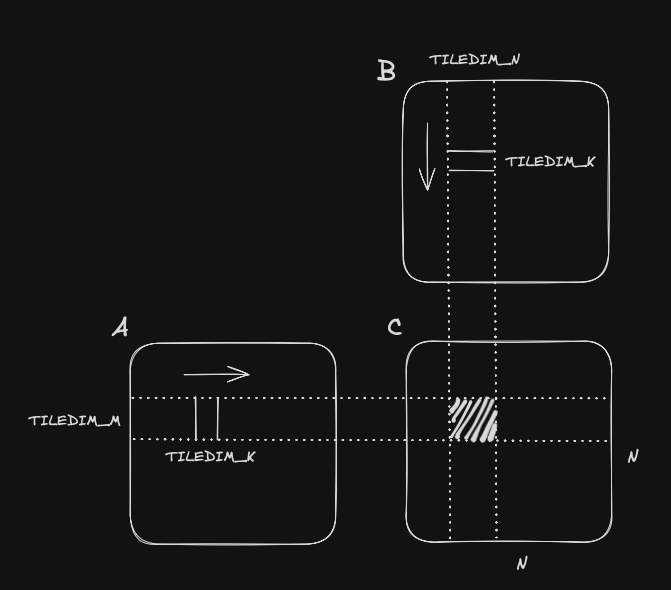
\includegraphics[width=0.85\linewidth]{block-tiling.png}
    \caption{Iterate over sub-block tiles to accumulate the outer product of
    submatrix $C$.}
    \label{fig:tiles}
\end{figure}

As shown in \cref{fig:outer}, each thread performs $\texttt{TILEDIM\_K}=32$ matrix
outer products. For each iteration over $K$, individual threads load 8 values from
block tile $A$ and 8 from block tile $B$ into registers. They then execute nested
loops to accumulate the $8\times8$ result locally before writing the final results
back to matrix $C$ in global memory. Computing the outer product exposes substantial
instruction-level parallelism (ILP) since there are no dependencies between
instructions here. Paired with the \texttt{\#pragma unroll} directive, we can guide
the compiler to perform loop unrolling to achieve this ILP while keeping the code
neat and flexible across various configurations.

\begin{figure}[t]
    \centering
    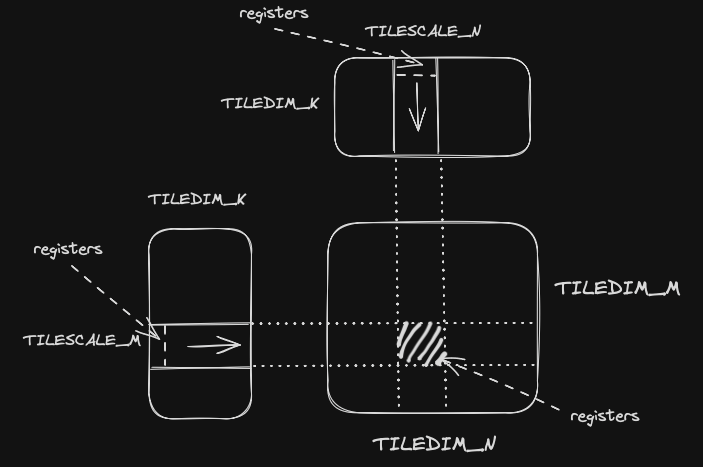
\includegraphics[width=0.95\linewidth]{thread-tile.png}
    \caption{Each thread calculates a
    $\texttt{TILESCALE\_M}\times\texttt{TILESCALE\_N}$ outer product.}
    \label{fig:outer}
\end{figure}

To handle edge cases where matrix dimensions aren't multiples of 128, we implement
bounds checking. During shared memory loading, we calculate global row and column
positions as the product of thread block coordinates and \texttt{TILEDIM},
validating these bounds before transferring data from global to shared memory. This
prevents result corruption from out-of-bounds data. Similarly, when writing results,
we check bounds to ensure memory safety at matrix edges. The code is shown in
\cref{fig:bounds-load,fig:bounds-write}.

\begin{figure}[t]
\begin{lstlisting}[style=cuda]
// populate the SMEM caches
#pragma unroll
for (uint loadOffset = 0; loadOffset < TILEDIM_M; loadOffset += strideA) {
    const uint globalRowA = globalRowOffset + innerRowA + loadOffset;
    const uint globalColA = bkIdx + innerColA;
    As[innerRowA + loadOffset][innerColA] =
        (globalRowA < N && globalColA < N)
            ? A[(innerRowA + loadOffset) * N + innerColA]
            : 0.0f;
}
#pragma unroll
for (uint loadOffset = 0; loadOffset < TILEDIM_K; loadOffset += strideB) {
    const uint globalRowB = bkIdx + innerRowB + loadOffset;
    const uint globalColB = globalColOffset + innerColB;
    Bs[innerRowB + loadOffset][innerColB] =
        (globalRowB < N && globalColB < N)
            ? B[(innerRowB + loadOffset) * N + innerColB]
            : 0.0f;
}
__syncthreads();
\end{lstlisting}
    \caption{Bounds checking when populating shared memory.}
    \label{fig:bounds-load}
\end{figure}

\begin{figure}[t]
\begin{lstlisting}[style=cuda]
// write out the results
#pragma unroll
for (uint resIdxM = 0; resIdxM < TILESCALE_M; ++resIdxM) {
#pragma unroll
    for (uint resIdxN = 0; resIdxN < TILESCALE_N; ++resIdxN) {
        const uint tileRow = threadRow * TILESCALE_M + resIdxM;
        const uint tileCol = threadCol * TILESCALE_N + resIdxN;
        if (globalRowOffset + tileRow < N &&
            globalColOffset + tileCol < N) {
            C[tileRow * N + tileCol] =
                threadResults[resIdxM][resIdxN];
        }
    }
}
\end{lstlisting}
    \caption{Bounds checking when writing results back to $C$.}
    \label{fig:bounds-write}
\end{figure}

Our development progressed through several stages. We started with shared memory
optimization, achieving a 50\% improvement over the naive kernel. We then implemented
1-D block tiling where each thread calculated a column of results, nearly doubling
performance. The transition to
two-dimensional block tiling was the hardest as we misunderstood the definitions of
blocks and tiles. We tried various configurations but performance dropped
significantly below that of 1-D block tiling. We believe it is due to bad coalesced
loads when loading to shared memory and performing too many computations per thread.
Thankfully, we clarified with TA Thomas during office hours that a block tile should
represent the values computed by an entire thread block. With this insight and
guidance from CUTLASS~\cite{cutlass} and Simon Boehm's blog~\cite{boehm}, we
successfully implemented our final solution.

\section{Results}
\label{sec:results}

\begin{figure*}[t]
    \centering
    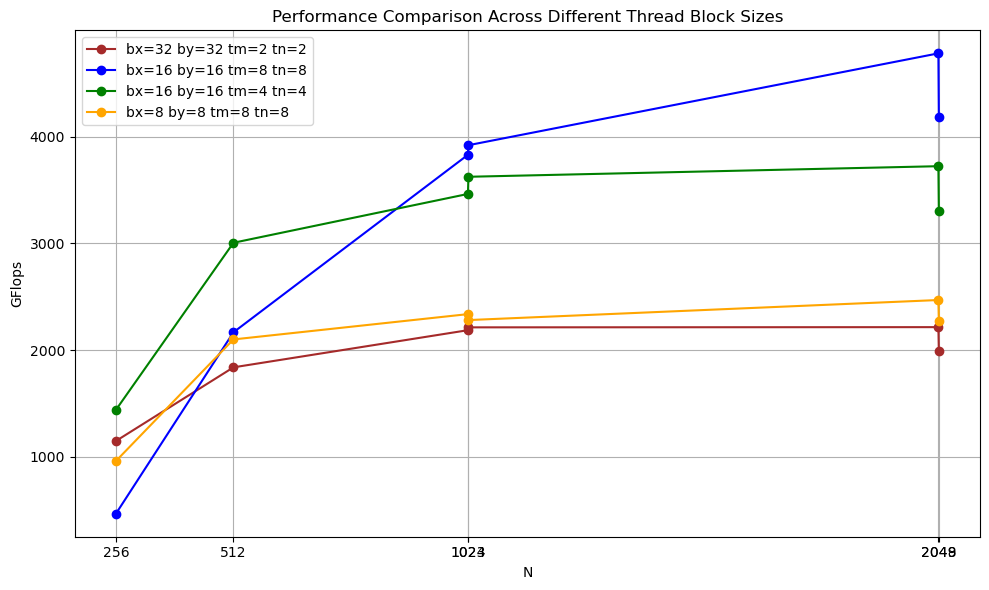
\includegraphics[width=0.72\textwidth]{perf-configs.png}
    \caption{Performance across various block dimensions and tile scales.}
    \label{fig:blockdims}
\end{figure*}

Throughout this section, we use the shorthand $T_M$, $T_N$, and $T_K$ for
\texttt{TILEDIM\_M}, \texttt{TILEDIM\_N}, and \texttt{TILEDIM\_K}; $B_x$ and $B_y$ for
the block dimensions \texttt{BLOCKDIM\_X} and \texttt{BLOCKDIM\_Y}; and $S_N$ for the
tile scale \texttt{TILESCALE\_N}.

\paragraph{(a) Configuration and access-pattern constraints.}
We fix $T_K = 32$, which means for each block tile, we divide $N$ into $N/T_K$
subtiles of $A$ of size $T_M \times T_K$, and in each iteration, we perform the outer
product $A_{T_M:N} \otimes B_{N:T_N}$.

The thread block and tile sizes are limited by the access pattern of $A$ when loading
into shared memory:
\begin{equation*}
B_x \times B_y \geq T_K.
\end{equation*}
Similarly for $B$:
\begin{equation*}
B_x \times B_y \geq T_N = S_N \times B_y.
\end{equation*}
The above equations can be simplified to:
\begin{equation*}
B_x \geq S_N.
\end{equation*}

\paragraph{(b) Occupancy analysis.}
Based on \cref{fig:blockdims}, the optimal thread block size is $16\times16$ across
all $N$. However, we observed some irregular performance behaviors when $N=256$. We
analyze the potential reasons for the performance differences from the perspective of
the number of warps and the possible maximum occupancy, as summarized in
\cref{tab:occupancy}.

\begin{table*}[t]
\centering
\caption{Occupancy analysis for several thread-block and tile configurations at
$N=256$ on the NVIDIA T4.}
\label{tab:occupancy}
\small
\begin{tabular}{@{}l c c c c c c c@{}}
\toprule
\textbf{Configuration} & \textbf{Tile Dim.} & \textbf{Thread Blocks} &
\textbf{Threads/Block} & \textbf{Threads} & \textbf{Regs/Thread} &
\textbf{Warps} & \textbf{Max Occ.} \\
\midrule
\texttt{bx=32 by=32 tm=2 tn=2} & 64  & 16 & 1024 & 16384 & 8  & 512 & 100\% \\
\texttt{bx=16 by=16 tm=8 tn=8} & 128 & 4  & 256  & 1024  & 80 & 32  & 80\%  \\
\texttt{bx=8 by=8 tm=8 tn=8}   & 64  & 16 & 64   & 1024  & 80 & 32  & 80\%  \\
\texttt{bx=16 by=16 tm=4 tn=4} & 64  & 16 & 256  & 4096  & 24 & 128 & 100\% \\
\bottomrule
\end{tabular}
\end{table*}

One intuitive explanation for why the configurations \texttt{bx=32,by=32,tm=2,tn=2}
and \texttt{bx=16,by=16,tm=4,tn=4} perform better at $N=256$ is that they require more
warps, which leads to more concurrent SM usage.

The second reason could be the limitation of register file size. For the
configurations \texttt{bx=16,by=16,tm=8,tn=8} and \texttt{bx=8,by=8,tm=8,tn=8}, each
thread utilizes $8 + 8 + 8\times8 = 80$ registers. The NVIDIA T4 GPU supports a
maximum of 256\,KB register files (equivalent to $64\text{K}$ float registers) per SM
and a maximum of 32 concurrent warps per SM.

For this implementation, the register file size becomes the limiting factor for
occupancy when $N$ is large because 32 warps would require:
\begin{equation*}
32\ \text{warps} \times 32\ \text{threads} \times 80\ \text{regs} = 81{,}920\
\text{registers},
\end{equation*}
which exceeds the maximum of $64\text{K}$ float registers. As a result, the maximum
number of active warps is given by:
\begin{equation*}
\frac{\text{total registers}}{\text{registers per warp}}
= \frac{64\text{K}}{80 \times 32} = 25.6\ \text{warps},
\end{equation*}
which leads to an occupancy of:
\begin{equation*}
25.6 / 32 \approx 80\%.
\end{equation*}
Thus, the SM is underutilized at approximately 80\% occupancy due to register
limitations. The total shared memory size is
$32 \times 16 \times 8 \times 2 \times 4\,\text{B} = 32\,\text{KB}$, which is within
the 64\,KB limitation.

For the configurations \texttt{bx=32,by=32,tm=2,tn=2} and
\texttt{bx=16,by=16,tm=4,tn=4}, the register file size is no longer a limitation to
occupancy; the occupancy is 100\%.

We noticed that high occupancy is not always needed to reach high performance when
the arithmetic intensity $q$ is small or large. $q$ is given by:
\begin{equation*}
q = \frac{f}{m},
\end{equation*}
where $f$ is the number of floating point operations, which is $2N^3$, and $m$ is the
number of memory operations. Each block tile loads $N(T_M + T_N)$ values from matrices
$A$ and $B$ into shared memory \texttt{As} and \texttt{Bs}, and the number of block
tiles is $N^2/(T_M T_N)$. We also perform $N^2$ store operations back to global
memory. Thus, we can simplify $q$ as:
\begin{equation*}
q = \frac{2N^3}{\dfrac{2N^3(T_M + T_N)}{T_M T_N} + N^2}
  = \frac{2N\,T_M T_N}{N(T_M + T_N) + T_M T_N}.
\end{equation*}
If we consider the square cases where $T_M = T_N$, we can simplify $q$ as:
\begin{equation*}
q = \frac{2N\,T_M}{2N + T_M}.
\end{equation*}
When $T_M$ is large, we become compute-bound and higher occupancy would not lead to
better throughput, as explained in the cusp behavior described by
Volkov~\cite{volkov_occupancy}. For the configuration \texttt{bx=16,by=16,tm=8,tn=8},
it has the highest $T_M$ of 128, yet it outperforms other configurations despite its
lower occupancy.

\paragraph{(c) Peak performance by matrix size.}
\Cref{tab:peakgf} documents the peak GFlops achieved and the corresponding thread
block size for each matrix size.

\begin{table}[t]
\centering
\caption{Peak GFlops and the corresponding thread block size for each matrix size.}
\label{tab:peakgf}
\small
\begin{tabular}{@{}l r l@{}}
\toprule
\textbf{$N$} & \textbf{Peak GF} & \textbf{Thread Block Size} \\
\midrule
256  & 1148.9 & \texttt{bx=16 by=16 tm=4 tn=4} \\
512  & 2166.9 & \texttt{bx=16 by=16 tm=8 tn=8} \\
1023 & 3829.8 & \texttt{bx=16 by=16 tm=8 tn=8} \\
1024 & 3919.6 & \texttt{bx=16 by=16 tm=8 tn=8} \\
2048 & 4779.9 & \texttt{bx=16 by=16 tm=8 tn=8} \\
2049 & 4181.0 & \texttt{bx=16 by=16 tm=8 tn=8} \\
\bottomrule
\end{tabular}
\end{table}

\section{Comparison to Naive}

\begin{figure}[t]
    \centering
    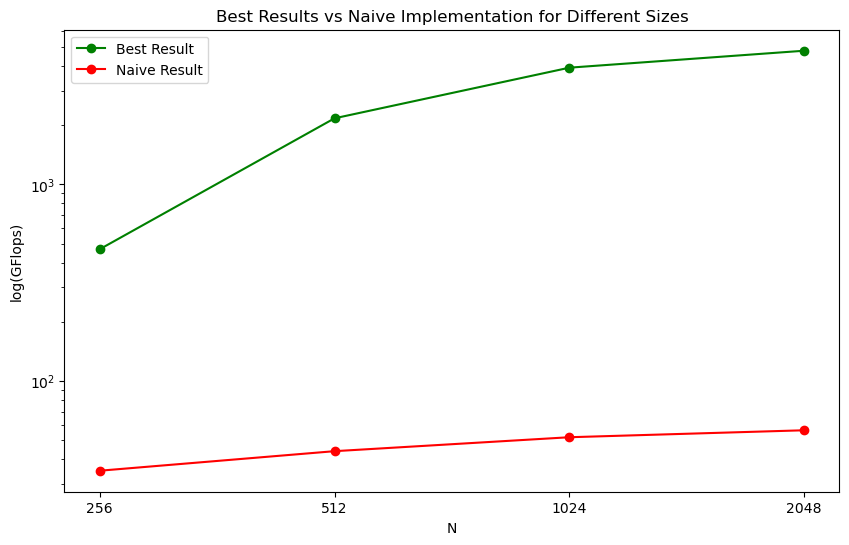
\includegraphics[width=0.9\linewidth]{vs-naive-gflops.png}
    \caption{$\log(\text{GFlops})$ comparison with the naive implementation.}
    \label{fig:lognaive}
\end{figure}

\begin{figure}[t]
    \centering
    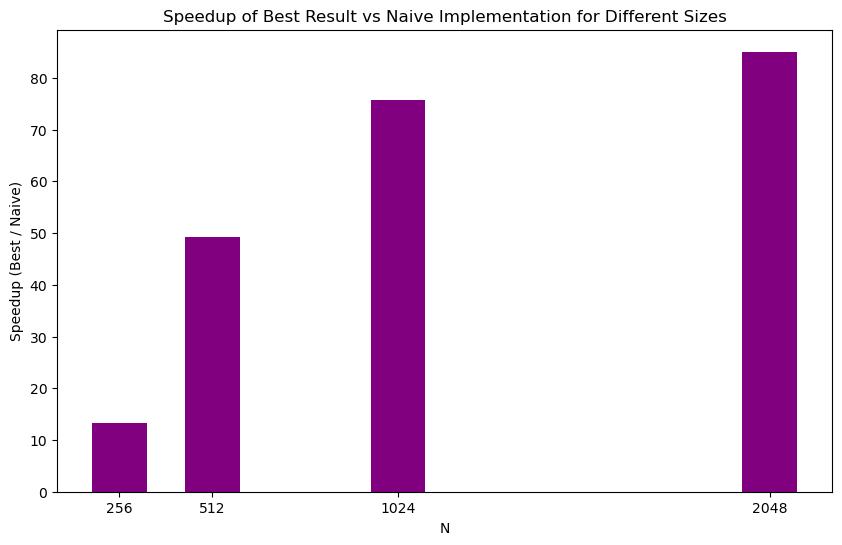
\includegraphics[width=0.9\linewidth]{vs-naive-speedup.png}
    \caption{Speedup over the naive implementation.}
    \label{fig:speedup}
\end{figure}

\Cref{fig:lognaive} compares the throughput of our kernel against the naive
implementation on a logarithmic scale, and \cref{fig:speedup} shows the corresponding
speedup.

\section{Analysis}

\begin{figure*}[t]
    \centering
    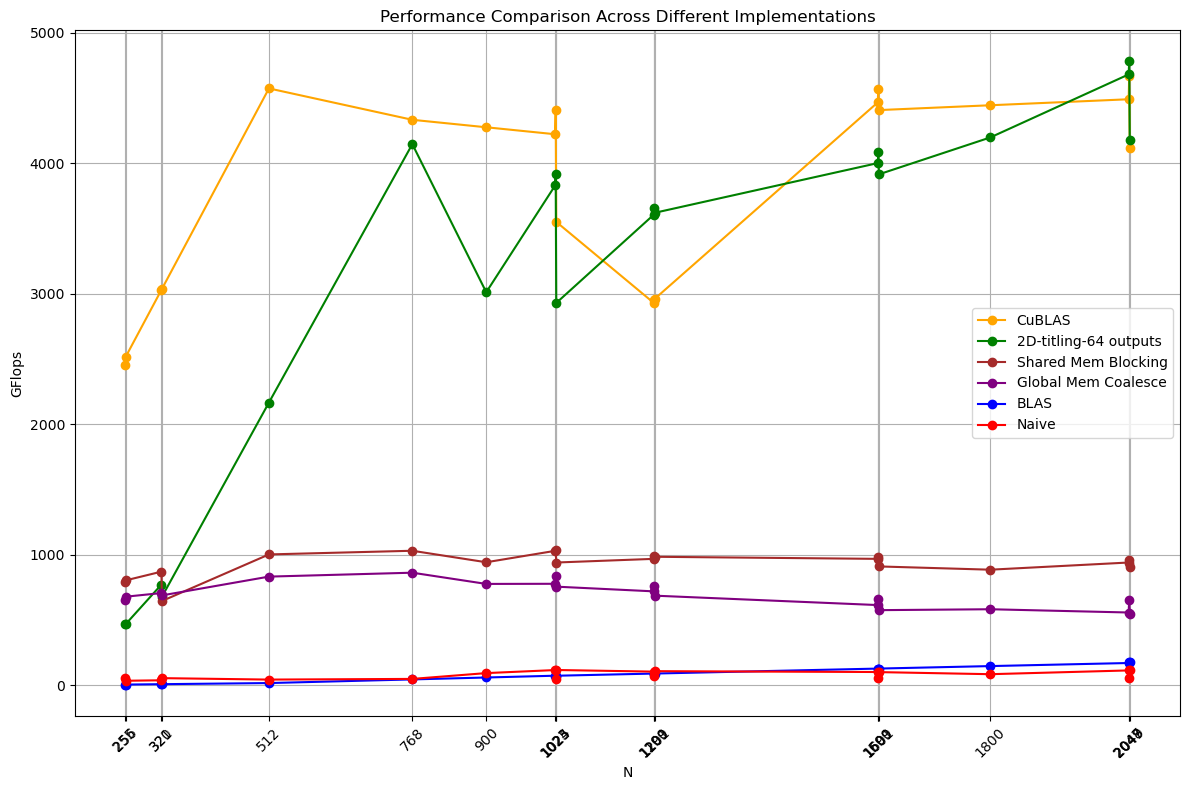
\includegraphics[width=0.72\textwidth]{perf-implementations.png}
    \caption{Performance across different implementations.}
    \label{fig:impls}
\end{figure*}

\paragraph{(a) Performance across implementations.}
\Cref{fig:impls} shows performance across our different implementations.

\paragraph{(b) Resemblance to cuBLAS.}
We noticed that the performance curve of our 2D-tiling-64-outputs method closely
resembles that of cuBLAS, with both showing fluctuations before converging to around
4000+ GFlops. One possible explanation for this similarity is that both methods are
based on the block-tile approach.

\paragraph{(c) Performance anomalies.}
We noticed two unusual behaviors in performance.

\smallskip
\noindent\emph{1) Performance degradation when $N$ is not a multiple of 128.}
Our 2D-tiling-64-outputs implementation and cuBLAS exhibit a significant performance
drop when the matrix size $N$ is not a multiple of 128. In contrast, other
implementations, such as 1-D blocking and naive methods, show much less fluctuation.
This disparity arises because our implementation is more complex, involving additional
branching conditions that cause more overhead during control divergence.

During boundary checks, when we attempt to fill the \texttt{As} and \texttt{Bs}
matrices with zeros for out-of-bounds accesses, some threads within a warp follow
different execution paths. As a result, the GPU must re-execute the warp for threads
that take the alternate path, causing performance degradation. For example, $N=1024$
benefits from perfect tiling and memory alignment. However, $N=1023$ leads to slight
tiling imbalances, resulting in minor inefficiencies, while $N=1025$ suffers from both
uneven tiling and memory misalignment, significantly reducing warp utilization. This
results in a performance drop from over 3900 GFlops to around 2900 GFlops.

A similar performance drop occurs when $N=1199$, 1200, and 1201. However, all these
matrix sizes fail to reach good memory alignment, and there is minimal difference in
performance across these three values. The varying degrees of performance degradation
suggest using different tile sizes, with each matrix size resulting in a different
level of tiling inefficiency.

\smallskip
\noindent\emph{2) Performance degradation when $N$ is greater than 768.}
When $N>768$, we observe that performance no longer improves significantly and, in
some cases, even degrades for certain matrix sizes. One possible reason is that the
kernel is increasingly memory-bound as $N$ increases. Since we fixed our kernel to
compute an $8\times8$ block per thread, computational intensity ($q$) plateaus after
$N=1000$. We use the same formula for $q$ as in \cref{sec:results}, giving us a
sawtooth logarithmic graph shown in \cref{fig:qintensity}:
\begin{equation*}
q = \frac{2N^3}{\bigl\lceil N/T_M \bigr\rceil^2 \cdot 2N\,T_M + N^2}.
\end{equation*}
The shape of the graph confirms our hypothesis that the performance of our
matrix-multiply implementation does not scale linearly with $N$ and dips when $N$ is
not a multiple of \texttt{TILEDIM\_M}.

% Flush the full-width Fig. 8 before Fig. 9 so they stay in numerical order.
\FloatBarrier

\begin{figure}[t]
    \centering
    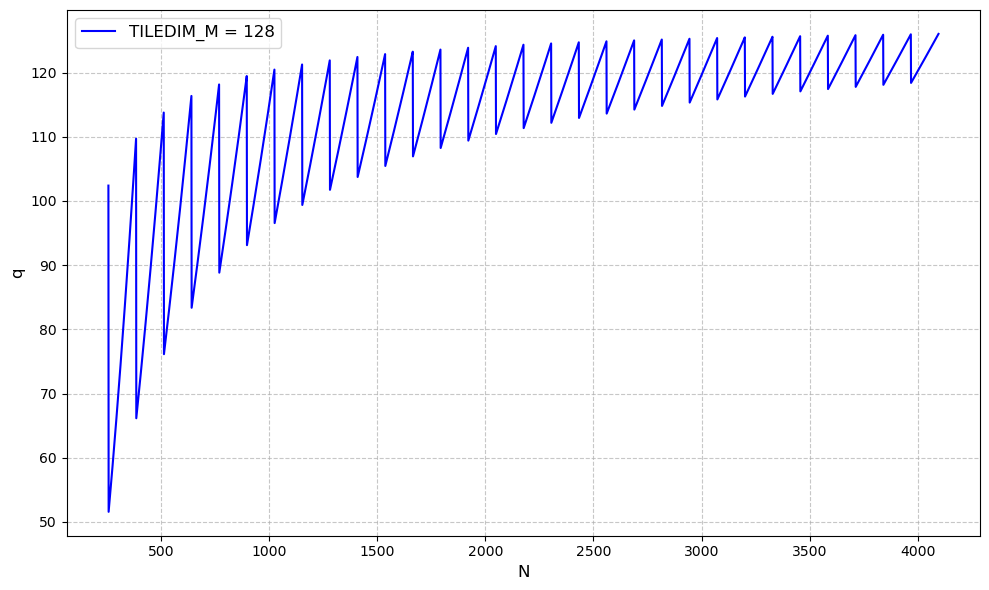
\includegraphics[width=0.9\linewidth]{arithmetic-intensity.png}
    \caption{Computational intensity of our kernel over $N$.}
    \label{fig:qintensity}
\end{figure}

\section{Calculations}

\paragraph{(a) Peak performance and arithmetic intensity.}
Peak performance is the total operations per second that a GPU can perform, assuming
all its cores execute their maximum number of ops per cycle, where frequency is
cycles per second per core. Thus,
\begin{equation*}
\begin{aligned}
\text{peak} &= \text{SMs} \times \tfrac{\text{cores}}{\text{SM}} \times \text{freq}
\times \tfrac{\text{ops}}{\text{cycle}}\\
&= 40 \times 64 \times (1.5\times10^{9}) \times 2\\
&= 7680\ \text{GFlops/s}.
\end{aligned}
\end{equation*}
For $n=2048$, we achieved 4779.9 GFlops. To calculate the arithmetic intensity $q$,
we divide the number of flops ($2n^3$) by the number of memory operations
($2n^3/\texttt{TILEDIM\_M}$ loads and $n^2$ stores), as shown in \cref{fig:calc1}.

\begin{figure}[t]
    \centering
    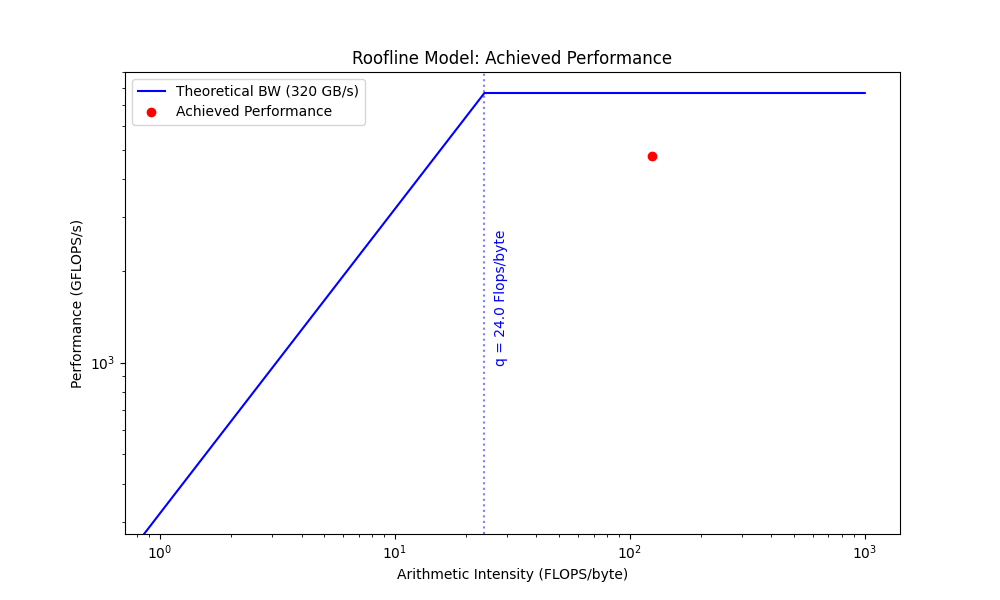
\includegraphics[width=0.85\linewidth]{roofline-achieved.png}
    \caption{Roofline model: achieved performance at $N=2048$ ($q = 24.0$
    Flops/byte).}
    \label{fig:calc1}
\end{figure}

\paragraph{(b) Effect of reduced memory bandwidth.}
$q = \text{peak flops} / \text{bandwidth} = 7680 / 320 = 24.0$ Flops/byte. The new
$q = 7680 / 220 = 34.9$ Flops/byte. The value of $q$ increased. This means we now need
greater arithmetic intensity to achieve peak performance, since we are limited by the
speed of memory operations (\cref{fig:calc2}).

\begin{figure}[t]
    \centering
    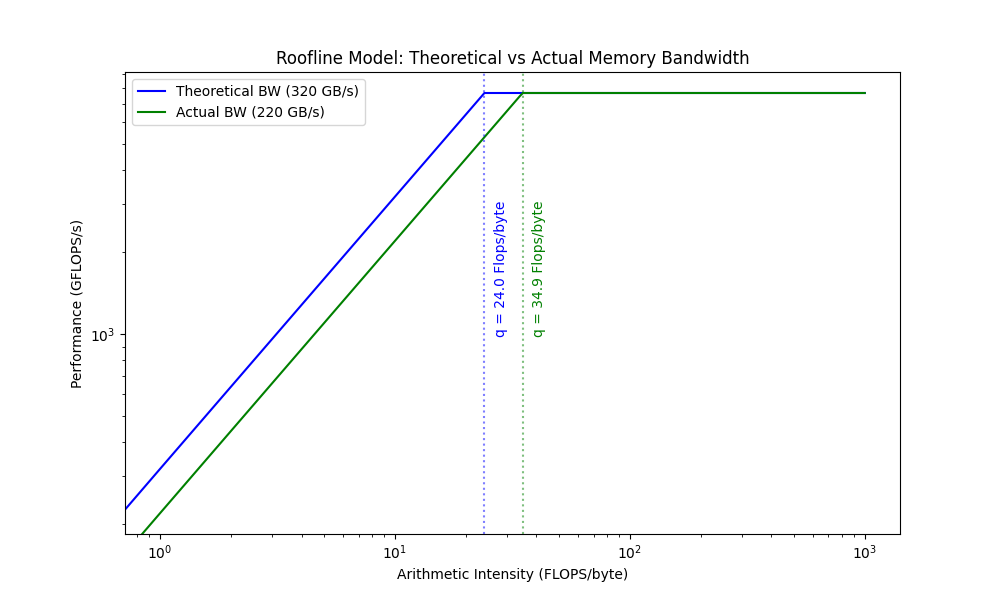
\includegraphics[width=0.85\linewidth]{roofline-bandwidth.png}
    \caption{Roofline model: theoretical versus actual memory bandwidth ($q = 24.0$
    versus $34.9$ Flops/byte).}
    \label{fig:calc2}
\end{figure}

\section{Potential Future Work}

Given more time, we would have explored interleaved computation as a potential
optimization. Since our current implementation already achieved strong performance, we
decided not to pursue it. This technique would have required a substantial departure
from our outer-product approach, which focuses on computing contiguous 2-D blocks. The
interleaved method would mean redesigning our thread block dimensions and tile sizes,
effectively requiring an architectural rethink rather than an incremental improvement
to our existing design.

\section{Extra Credit}

We created a non-square matrix multiplication kernel with the following header in
\texttt{mmpy\_kernel.cu}:
\begin{quote}
\small\ttfamily\raggedright
\_\_global\_\_ void matMulNonSquare(\\
\hspace*{1.5em}int M, int N, int K,\\
\hspace*{1.5em}\_FTYPE\_ *\_\_restrict\_\_ C,\\
\hspace*{1.5em}\_FTYPE\_ *\_\_restrict\_\_ A,\\
\hspace*{1.5em}\_FTYPE\_ *\_\_restrict\_\_ B)
\end{quote}
This required three changes to our original implementation. First, we updated the
outer loop bound from $N$ to $K$, since $K$ represents the shared dimension between
matrices $A$ and $B$ used to iterate the sub-block tiles (refer to \cref{fig:tiles}).
Second, we modified the shared memory loading bounds to check against $M$ for matrix
$A$ and $N$ for matrix $B$. Finally, when writing results back to matrix $C$, we
updated our bounds checking to compare the global row offset against $M$ and the global
column offset against $N$, since the output is now an $M\times N$ matrix.

To optimize our non-square matrix multiplication kernel, we could implement several
changes. Instead of using fixed $128\times128$ tile sizes, we could dynamically adjust
tile dimensions $M$, $N$, and $K$. For example, if $M$ is much larger than $N$, we can
scale \texttt{TILEDIM\_M} by a larger factor (using \texttt{TILESCALE\_M}) up to the
shared memory limit. Essentially, our outer product dimensions would be proportional
to $M$ and $N$, maximizing the amount of work done per thread. When $K$ is much larger
than $M$ or $N$, we could increase \texttt{TILEDIM\_K} (while adjusting other
parameters) to maximize shared memory utilization. These changes would enable the
matrix multiplication computation to remain highly performant across varying input
sizes.

\begin{thebibliography}{9}

\bibitem{volkov_latency}
V. Volkov. \textit{Understanding Latency Hiding on GPUs}. Ph.D. thesis, University of
California, Berkeley, Technical Report UCB/EECS-2016-143, 2016.
\url{https://www2.eecs.berkeley.edu/Pubs/TechRpts/2016/EECS-2016-143.html}.

\bibitem{volkov_occupancy}
V. Volkov. Better performance at lower occupancy. In \textit{GPU Technology Conference
(GTC)}, 2010.
\url{https://www.nvidia.com/content/gtc-2010/pdfs/2238_gtc2010.pdf}.

\bibitem{cutlass}
NVIDIA. CUTLASS: Fast linear algebra in CUDA C++. NVIDIA Technical Blog.
\url{https://developer.nvidia.com/blog/cutlass-linear-algebra-cuda/}.

\bibitem{tiledmm}
Must know technique in GPU computing: Tiled matrix multiplication in CUDA C.
\url{https://www.youtube.com/watch?v=Q3GgbfGTnVc}.

\bibitem{boehm}
S. Boehm. How to optimize a CUDA matmul kernel for cuBLAS-like performance: A worklog.
\url{https://siboehm.com/articles/22/CUDA-MMM}.

\end{thebibliography}

\balance

\end{document}
